\chapter{Background}

In this chapter we cover several elements of background research needed for the project. We introduce the idea of political bias (Section \ref{sec:political-bias}), and look at existing datasets of news content annotated by political bias (Section \ref{sec:existing-news-datasets}), followed by machine learning methods that have been employed to detect bias in news (Section \ref{sec:detecting-political-bias-in-news}). We then introduce Reddit (Section \ref{sec:reddit}) and the idea of readership bias (Section \ref{sec:readership-bias}), and explore related work in detecting political readership bias on social media. Finally, we introduce transfer learning (Section \ref{sec:transfer-learning}) and specifically previous work in domain adaptation (Section \ref{subsec:domain-adaptation}).

\section{Political bias} \label{sec:political-bias}

Discussions on political bias are mainly focused on whether a particular news source is left-wing or right-wing. The definition of each is not clear-cut, and the boundaries between what constitutes left-wing thought and right-wing thought varies between countries, and between historical periods and today.

A YouGov survey \cite{yougov} in 2019 found that issues in the UK that matter most to left-wing voters include remaining in the EU, opposing the use of nuclear weapons, increasing the minimum wage, supporting industry nationalisation and increasing wealth tax, whereas right-wing voters support the opposite viewpoint. In the USA \cite{diffen} left-wing viewpoints include expanding government healthcare programs and social security, tightening environmental regulation, increasing corporation tax, expanding amnesty to undocumented immigrants, and again right-wing viewpoints are in opposition.

Overarching themes that can be drawn include that left-wing thought more often than not supports expanding the role of government, whereas right-wing thought advocates for smaller government. Economically, left wing voters tend to support tight financial regulation, however right wing voters support less regulation in favour of a free market economy, and left wing voters often support globalisation and stronger international ties with other countries whereas right wing voters are more sceptical of globalisation and may prefer protectionism.

Of course, political bias in text can be extremely nuanced, hence the interest in using automatic natural language processing methods for detection.

\section{Existing news datasets} \label{sec:existing-news-datasets}

In this section we look at some existing datasets of news sources and news articles that have been annotated by political bias.

\subsection{Media Bias/Fact Check}

Media Bias/Fact Check (MBFC) provides a list of over 3500 news sources, annotated with their respective political bias leanings \cite{mbfc}. The news sources covered are mostly US-based, and include mainstream and non-mainstream media - examples include CNN, Fox News, Breitbart, Bloomberg, and many more.

MBFC has a team of volunteers who manually assess and assign scores per-source based on content from their articles. Each source is scored from 1-10 on the four following categories: biased wording/headlines, factuality/well-sourced information, story portrayal, and political affiliation \cite{MBFC-methodology}. The scoring mechanism is shown in Table \ref{tab:MBFC-scoring}.

\begin{table}[ht]
    \centering
    \begin{tabular}{|c|c|c|c|}
        \hline
        0-2 & 2-5 & 5-8 & 8-10 \\
        \hline
        Least Biased & Slightly Biased & Moderately Biased & Extremely Biased \\
        \hline
    \end{tabular}
    \caption{MBFC scoring mechanism}
    \label{tab:MBFC-scoring}
\end{table}

The scores across the 4 categories are averaged to produce an overall score for each news source. Note that this scale only measures the degree of bias and not the direction of bias (e.g. left/right wing) - this is manually classified by MBFC's volunteers. MBFC also produces a detailed report giving more information about each source's particular traits, for example the following is a sample from the report on CNN:

\begin{quote}
\textit{``...we rate CNN left biased based on editorial positions that consistently favors the left, while straight news reporting falls left-center through bias by omission. We also rate them Mixed for factual reporting due to several failed fact checks by TV hosts. However, news reporting on the website tends to be properly sourced with minimal failed fact checks.''} \cite{MBFC-CNN}
\end{quote}

Note since most catalogued news sources are based in the USA, this scale is centred heavily on the US political scale.

\subsection{News-Media-Reliability} \label{subsec:news-media-reliability}

Baly et al., as part of their analysis on detecting political bias \cite{baly-emnlp18}, created the News-Media-Reliability dataset \cite{news-media-reliability}, a collection of engineered features from 1066 news sites, with political bias annotations provided by Media Bias/Fact Check. Sites are categorised according to 7 labels: \textit{extreme-left, left, center-left, center, center-right, right} and \textit{extreme-right}. The dataset features include textual features from each site's article content and its headlines, as well as information from the site's Twitter page and Wikipedia page (if they exist), and its Alexa web traffic rank. The full collection of features is given in Table \ref{tab:nmr-features}.

\begin{table}[h!]
    \centering
    \begin{tabular}{|c|c|c|}
        \hline
        \textbf{Category} & \textbf{Feature} & \textbf{Description} \\
        \hline
        Site traffic & alexa & Alexa ranking \\
        \hline
        URL & url\_structure & Site URL \\
        \hline
        \multirow{2}{4em}{Articles} & articles\_title\_glove & Article headline features \\
        & articles\_body\_glove & Article body features \\
        \hline
        \multirow{7}{4em}{Twitter} & has\_twitter & Whether site has Twitter or not \\
        & twitter\_created\_at & Year Twitter account was created \\
        & twitter\_description & Twitter account biography \\
        & twitter\_engagement & Twitter user engagement metrics \\
        & twitter\_haslocation & Whether site has location in their Twitter biography or not \\
        & twitter\_urlmatch & Whether Twitter account contains a link to the site URL \\
        & twitter\_verified & Whether Twitter account is verified or not \\
        \hline
        \multirow{4}{4em}{Wikipedia} & wikipedia\_categories & Wikipedia page categories features \\
        & wikipedia\_content & Wikipedia page content features \\
        & wikipedia\_summary & Wikipedia page summary features \\
        & wikipedia\_toc &  Wikipedia page table of contents features \\
        \hline
    \end{tabular}
    \caption{Engineered features in the News-Media-Reliability dataset}
    \label{tab:nmr-features}
\end{table}

The articles\_title\_glove and articles\_body\_glove features aren't actually the text content of the headline/body, but a set of 141-dimensional custom features relating to the structure of the text, sentiment scores, language bias analysis and also complexity of the text, expressed as 141-vectors. More details are given in Baly et al. \cite{baly-emnlp18}. The Wikipedia features are word2vec word embeddings of the corresponding text (see Section \ref{subsec:word-embeddings} for more detail). Overall this featureset is fairly comprehensive, as it includes a well-rounded representation of a news source's article content plus content taken from the source's online presence.

\section{Detecting political bias in the news} \label{sec:detecting-political-bias-in-news}

In this section we will look at examples of techniques that have been applied to detect political bias in the news with NLP.

\subsection{Word embeddings} \label{subsec:word-embeddings}

In order to run machine learning models on words, they must first be converted into feature vectors. Word embeddings are a representation of words in a finite-dimensional vector space, such that the word embeddings of words that are semantically similar are closer to each other in the vector space. Word embeddings can be learnt manually by training a neural network to generate them using an embedding layer, or pre-trained models can be used such as Google's word2vec \cite{word2vec}, or GloVe \cite{glove}.

Word embeddings by themselves have been used to analyse bias in text. Bolukbasi et al. \cite{gender-bias-word-embeddings} use the cosine similarity between averaged word embeddings of Google News articles to detect gender bias, and Gordon et al. \cite{political-bias-word-embeddings} use the same idea on tweets to detect political bias. However, they are most often used as a pre-processing technique for machine learning models.

\subsection{SVMs} \label{subsec:svms}

Support vector machines (SVMs) are supervised models that can be used for both classification and regression. In the classification case, finding the decision boundary between classes in feature space is formulated as an optimisation problem, which the classifier approximates using gradient descent. We can change the function being used to model the decision boundary, called the kernel. A common kernel used instead of the standard linear one is the radial basis function (RBF) kernel. This is useful for modelling classes which occur in spherical clusters rather than with straight-line boundaries.

Baly et al. \cite{baly-emnlp18} trained an SVM classifier to detect political bias in the News-Media-Reliability dataset. They used an RBF kernel, and provided F1 and accuracy scores for classifiers trained on individual News-Media-Reliability features (see Table \ref{tab:nmr-features}) as well as groups of features, compared to a `majority' baseline that always predicts the majority class in the dataset (i.e. the modal class). They achieved a highest F1 score of 61.31\% and accuracy of 68.86\% after merging small classes. The code and the dataset for this study are open-source and available on GitHub, making it easy to reproduce the paper's results. The authors do not compare SVMs with any other classifiers, providing ample opportunity for future work.

\subsection{Ensemble classifiers} \label{subsec:ensemble-classifiers}

Ensemble classifiers involve aggregating predictions from a group of classifiers, called \textit{base learners}, in order to improve accuracy when compared to individual classifiers. In the classification case, aggregation usually involves taking a majority vote from the base learners' predictions. In order for ensemble learning to work, the base learners should ideally be uncorrelated (that is, there shouldn't be any patterns between predictions of any two base learners for the same training samples).

Two common ensemble learning techniques are \textit{bagging} and \textit{boosting}. Bagging (\underline{B}ootstrap \underline{Agg}regating) involves bootstrapping say, $ T $ new training datasets from an original dataset, and training $ T $ independent base learners on each new dataset. During inference time, a majority vote of predictions from each base learner is used to form an overall prediction. A popular bagging technique is a random forest, which is a ensemble of decision trees.

Boosting involves training base learners serially on the same training set, instead of in parallel as with bagging. In Adaboost, the first boosting algorithm created, any mis-classified examples from one learner are upweighted for the next learner, meaning an ensemble of the base learners learns a good representation of all the data. Adaboost uses decision stumps as base learners (decision trees of depth 1). In a more modern technique called gradient-boosted trees, full decision trees are used as base learners, and residual errors from previous learners are factored in to each learner's training.

Ensemble classifiers have not been extensively explored for the problem of detecting political bias. Voong et al. \cite{voong} compared gradient-boosted forests to Naive Bayes classifiers, SVMs, and logistic regression in detecting political bias of tweets, finding gradient-boosted forests gave the highest accuracy and F1 scores.

\subsection{BERT}

BERT (Bidirectional Encoder Representations from Transformers) \cite{bert} is a transformer-based model developed for natural language processing purposes. Transformer networks can learn contexts across extremely long sentences and paragraphs, and also enables bi-directional training that allows transformers to learn context even more deeply.

BERT is a stack of encoder models that utilises semi-supervised learning. This means BERT models are often pre-trained for use with a particular language, e.g. English, and then fine-tuned for a particular NLP task. Fine-tuning is often fast, as the main bulk of training is performed in pre-training. Pre-training involves two tasks:
\begin{itemize}
    \item \textbf{Masked Language Modelling (MLM)} - random words in the input text are replaced with \texttt{[MASK]} tokens, and BERT is trained to predict the missing words. This helps BERT understand bi-directional context between words in a single sentence.
    \item \textbf{Next Sentence Prediction (NSP)} - BERT takes in two sentences A and B, and determines whether sentence B actually follows sentence A in the text or not. This helps BERT understand context across lots of sentences.
\end{itemize}

A diagram of BERT during both pre-training and fine-tuning is shown in Figure \ref{fig:bert-pretraining-finetuning}. During pre-training, BERT generates its own contextualised word embeddings which it then uses throughout the encoder stack. BERT models come in varying sizes, the most popular being `base' and `large'. The base model contains 12 layers with each hidden layer containing 768 neurons, and gives 110M trainable parameters overall. The large model contains 24 layers each with 1024 neurons, and gives 340M trainable parameters. The large model often produces better results than base for popular benchmarks in sequence classification, question answering and other common NLP tasks, however it requires much more memory to train.

\begin{figure}
    \centering
    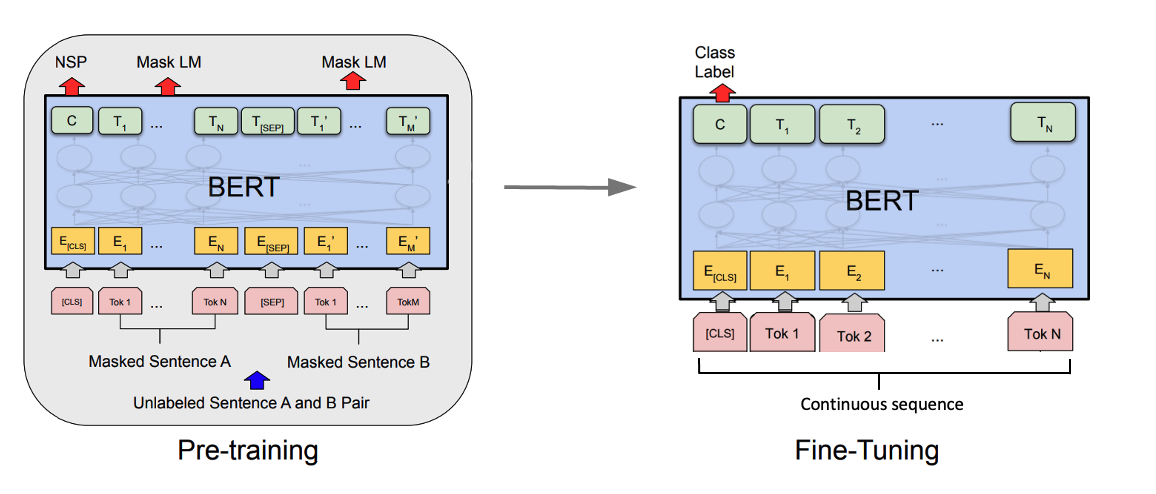
\includegraphics[scale=0.37]{0-img/bert-pretraining-finetuning.png}
    \caption{BERT pre-training and fine-tuning stages, in this case for sequence classification (edited from \cite{bert})}
    \label{fig:bert-pretraining-finetuning}
\end{figure}

Input sequences into BERT must first have special [CLS] and [SEP] tokens added to them. A [CLS] token denotes the beginning of the input sequence, and [SEP] tokens are added between sentences as markers for BERT. The input sequence is then converted to token IDs, segment IDs and attention IDs. For more information on these, see \cite{bert}.

Chun et al. \cite{chun} used BERT to simultanously detect political bias and detect trolls on Twitter, finding that the accuracy, precision and recall of the BERT model far surpassed those of the other models used (SVMs, standard neural networks and convolutional neural networks). They report a highest accuracy of 89\% for the bias detection task. The Bipartisan Press in their analysis \cite{bipartisan-press} found BERT performs much better at predicting both amount of bias and direction of bias than both LSTMs (long short-term memory networks) and ULMFiT (a transfer-learning-based model), as well as an ensemble model built from the two. They obtained even better results when using RoBERTa \cite{roberta}, a version of BERT that has been pre-trained for longer and with more data. Baly et al. \cite{baly-acl2020} used BERT contextualised word embeddings extracted from article text as an input feature to an SVM trained to detect bias. They report a highest F1 of 81.27\% and accuracy of 81.83\%, both much higher than for their earlier SVM classifier without BERT.

\section{Reddit} \label{sec:reddit}

Reddit is one of the most popular social media platforms today, with over 430 million active users as of April 2020 \cite{sattelberg}. Reddit is characterised by its unique `subreddits' feature: communities that any user can join in order to read posts, comment, and post themselves about a particular topic. Subreddits begin with `r/' followed by the topic name, for example popular subreddits include r/sports, r/astronomy, r/books and r/cooking. More politically-oriented subreddits include r/liberal, r/conservative, r/worldpolitics, r/ukpolitics, and many more. Reddit users can `upvote' or `downvote' any posts or comments, which increases/decreases their visibility to other users.

\begin{figure}
    \centering
    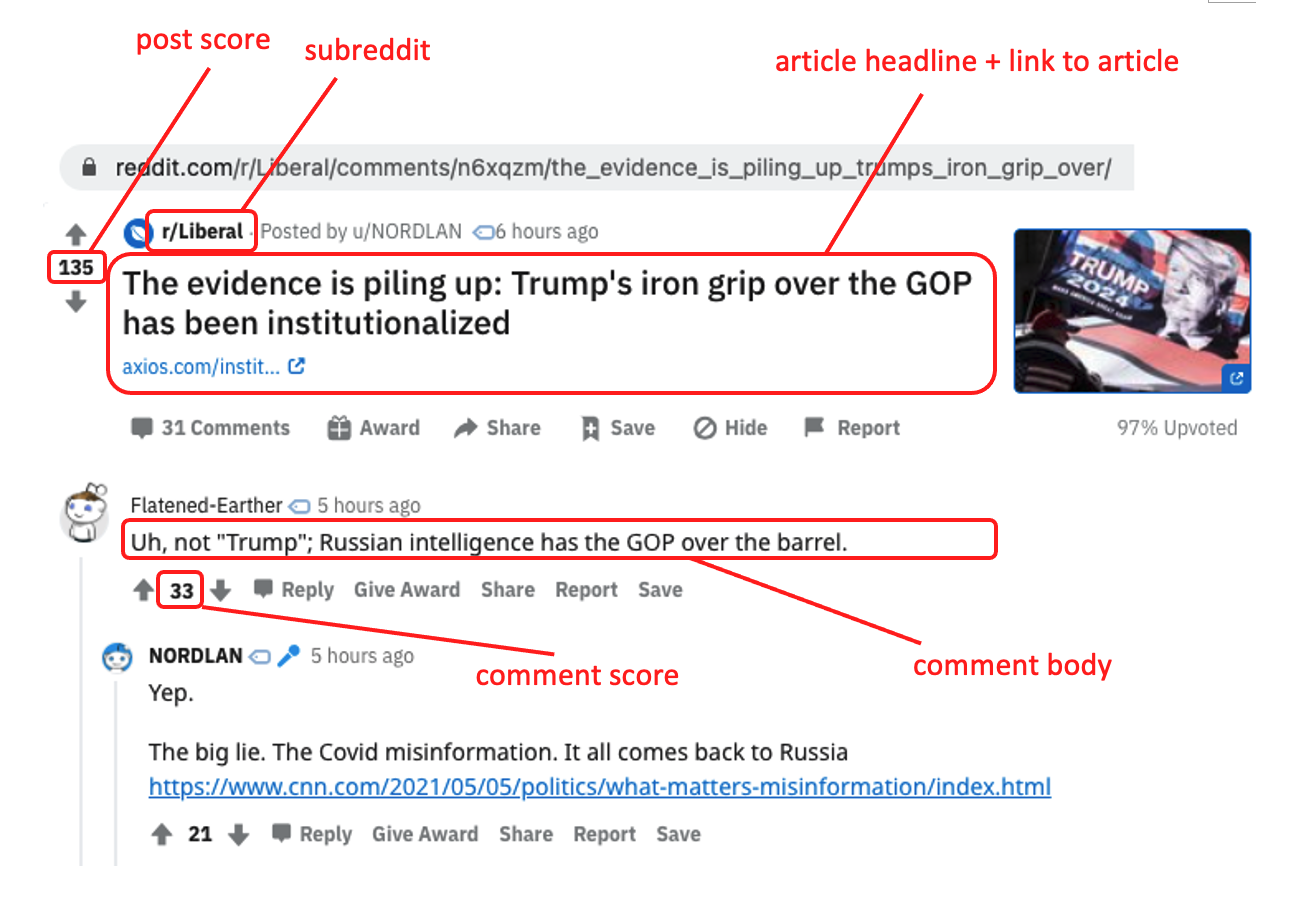
\includegraphics[scale=0.27]{0-img/annotated-reddit-post.png}
    \caption{The anatomy of a typical Reddit post}
    \label{fig:annotated-reddit-post}
\end{figure}

Figure \ref{fig:annotated-reddit-post} shows what a typical Reddit post looks like. The post and comment `scores' are simply the sum of any upvotes and downvotes that particular post or comment has - an upvote counts as +1, a downvote as -1. Reddit provides a `top posts' feature for each subreddit that allows users to search for the top posts by score in the last day/week/month/year.

A typical post on a political subreddit involves a link to a particular news article, and a comment stream with reactions from people who frequent that subreddit. Most often this will be the users that are actually subscribed to that subreddit, but occasionally there is discourse between subscribers and non-subscribers.

\subsection{Collecting Reddit data} \label{subsec:collecting-reddit-data}

Reddit data can be collected from the public Reddit API \cite{reddit-api}, or from online data dumps of Reddit posts such as the PushShift dataset \cite{pushshift}.

The Reddit API yields JSON files that describe any given subreddit, post, comment or user on the website. Examples of information exposed by the API include subreddit names, descriptions, post content, links to webpages referenced in posts, post scores, comment text and comment scores. The API also provides features to search for the most recent posts in a particular subreddit, and the top $ n $ posts in that subreddit in the last day/week/month/year. The API is most commonly accessed with the Python \texttt{praw} package \cite{praw}.

The PushShift dataset is a large data dump of Reddit posts, comments, subreddit information and more, assembled by Reddit user Jason Baumgartner. It is available online at \url{https://files.pushshift.io/reddit/} \cite{pushshift}. The dataset contains Reddit posts and Reddit comments arranged by month from June 2005 (the month Reddit was created) through to December 2019 - in total the dataset contains around 651 million posts and 5.6 billion comments. The dataset contains almost all the same information the Reddit API exposes, however one cannot fetch the top $ n $ posts in that subreddit at a particular point in time.

In terms of data annotated by political bias, there is a severe lack of published datasets of Reddit content in this format. Almost all papers exploring political bias on Reddit (see Section \ref{subsec:readership-bias-social-media}) do not make their data available publicly.

\section{Readership bias} \label{sec:readership-bias}

We define readership bias as the bias shown by audiences, rather than by a news source. A significant portion of readership bias research so far has focused on analysing the sentiment of readers - early work on this was done by Lin et al. \cite{lin}, who classified news articles by 8 different possible emotions expressed by the reader, recorded as reactions on Yahoo's website. Psychologist Paul Ekman popularised the existence of 6 basic emotions \cite{ekman}: happiness, sadness, anger, fear, disgust and surprise. Strapparava et al. \cite{strapparava} used this emotion model to detect sentiment analysis in news headlines with a Naive Bayes classifier. Tan \cite{chien-tan} also created a readership bias model based on the 6 emotions, and separately created a model to predict the distribution of Facebook Reactions on posts containing links to news articles.

\subsection{Detecting political readership bias on social media} \label{subsec:readership-bias-social-media}

Social media is increasingly becoming a hub for political discussion and discourse. Garimella \& Weber \cite{garimella} analysed the political polarisation of Twitter discussions over time using retweets and hashtags used by 670,000 Twitter users, finding that polarisation increased by around 10-20\% between 2009 and 2016. Rao et al. \cite{rao} used SVMs trained on n-gram features extracted from tweet text to predict the political affiliation of various Twitter users. Voong et al. \cite{voong} compared Naive Bayes classifiers, SVMs, logistic regression, and random forests with gradient boosting in predicting political polarity of tweets, also using an n-gram approach, finding logistic regression and random forests to give the highest accuracy and F1 scores, and Naive Bayes to give the worst.

Baly et al. \cite{baly-acl2020} interestingly used features taken from readers' Facebook and Twitter profiles as a predictor for a news source's political bias. Baly's model of thinking was that a source's audience characterises how biased that source is and in what direction (that is, readership bias determines bias in the source). This differs from the mainstream line of thinking, which is that bias in the source determines readership bias. It is hard to say which of these philosophies is `correct' - indeed there may be an element of both at play, that is news organisations will decide what to publish based on their target audience, and at the same time their target audience will change depending on what they publish.

Other social media platforms such as Reddit have been less explored. Kane \& Luo \cite{kane} carried out an exploration into political communities on Reddit, examining whether non-political subreddits still exhibit some unconscious political leaning. They did this by analysing comments across different posts within these subreddits and using Latent Dirichlet Allocation (LDA) to see which topics appear most frequently in each subreddit. This topic model was then used to train a classifier to predict the political bias of a subreddit, based on its most-common topics. They were able to achieve a highest accuracy of 85.2\% with an SVM classifier using n-gram features. Since LDA is an unsupervised method, Kane \& Luo didn't have to source any Reddit data annotated by political bias, which is extremely scarce.

Predicting support for specific political figures on social media is a popular task, especially during widely-publicised elections such as the 2016 and 2020 US elections. Massachs et al. \cite{massachs} predict support for Donald Trump using a combination of homophily and social feedback exhibited on r/The\_Donald, a popular subreddit centred around support for Donald Trump. They report a highest accuracy of 35.5\%, suggesting this problem is significantly more challenging than simply detecting left/right-wing bias. It is worth noting that the authors use participation in r/The\_Donald to annotate Reddit users as Trump supporters or not, suggesting they assume only Donald Trump supporters will post in r/The\_Donald. We examine this assumption in Chapter \ref{chap:reddit-data}.

\section{Transfer learning} \label{sec:transfer-learning}

Transfer learning is the study of training a machine learning model for a particular problem A, and applying the model to a different but related problem B. Transfer learning may be explored when it is hard obtaining suitable annotated training data for problem B, or because training for problem B would take too long otherwise.

One popular example of transfer learning is in BERT models - BERT is pre-trained on text from BookCorpus and English Wikipedia \cite{bert} for the tasks of masked language modelling and next sentence prediction, and is later fine-tuned for the target task at hand (which could be sentence classification, question answering, named entity recognition, etc.). Another popular form of transfer learning occurs in imaging problems, where CNNs pre-trained for image classification on ImageNet are then fine-tuned for other tasks such as object detection, image segmentation, or perhaps for further image classification.

In the following, we use notation similar to previous literature \cite{ruder} \cite{pan-survey} to formalise the theory of transfer learning:

A data domain $ \mathcal{D} $ can be formulated as a feature space $ \mathcal{X} $ accompanied by a probability distribution $ P(X) $ over the feature space. Intuitively, a domain is a set of data that exhibits a unique set of characteristics with respect to some feature space. In the real world, different textual domains include literary writing, scientific writing, news article text, tweets, etc. These will all exhibit a different distribution of features if we use a feature space of, say, $n$-dimensional word embeddings.

Given some domain $ \mathcal{D} = (\mathcal{X}, P(X)) $, a task $ \mathcal{T} $ is defined as a set of labels $ \mathcal{Y} $ and a prior (or `ground truth') label distribution $ P(Y) $. A classifier aims to learn the conditional probability distribution $ P(Y | X) $ from some training data $ \{x_i, y_i\}_{i=1}^{n} $.

Given a \textbf{source domain} $ \mathcal{D}_S $ and \textbf{source task} $ \mathcal{T}_S $, along with \textbf{target domain} $ \mathcal{D}_T $ and \textbf{target task} $ \mathcal{T}_T $, the goal of transfer learning is to learn the conditional distribution $ P_T (Y_T | X_T) $ in domain $ \mathcal{D}_T $.

\textit{Transductive transfer learning} is when the target task is the same as the source task (i.e. $ \mathcal{T}_S = \mathcal{T}_T $), however the source domain and target domain may vary, or labelled data may only be available in the source domain. Examples of transductive transfer learning include domain adaptation and cross-lingual learning. \textit{Inductive transfer learning} is when the two tasks are not the same, and labelled data for the target domain is often present. Examples of inductive transfer learning include multi-task learning and sequential transfer learning. 

\subsection{Domain adaptation} \label{subsec:domain-adaptation}

Domain adaptation (also known as cross-domain learning) is a specific case of transductive transfer learning. In this case the source task and target task are identical, however the source and target domains may be different, or labelled target data may not be available (in which case we perform \textit{unsupervised} domain adaptation). Figure \ref{fig:domain-adaptation} shows a typical domain adaptation problem.

\begin{figure}[ht]
    \centering
    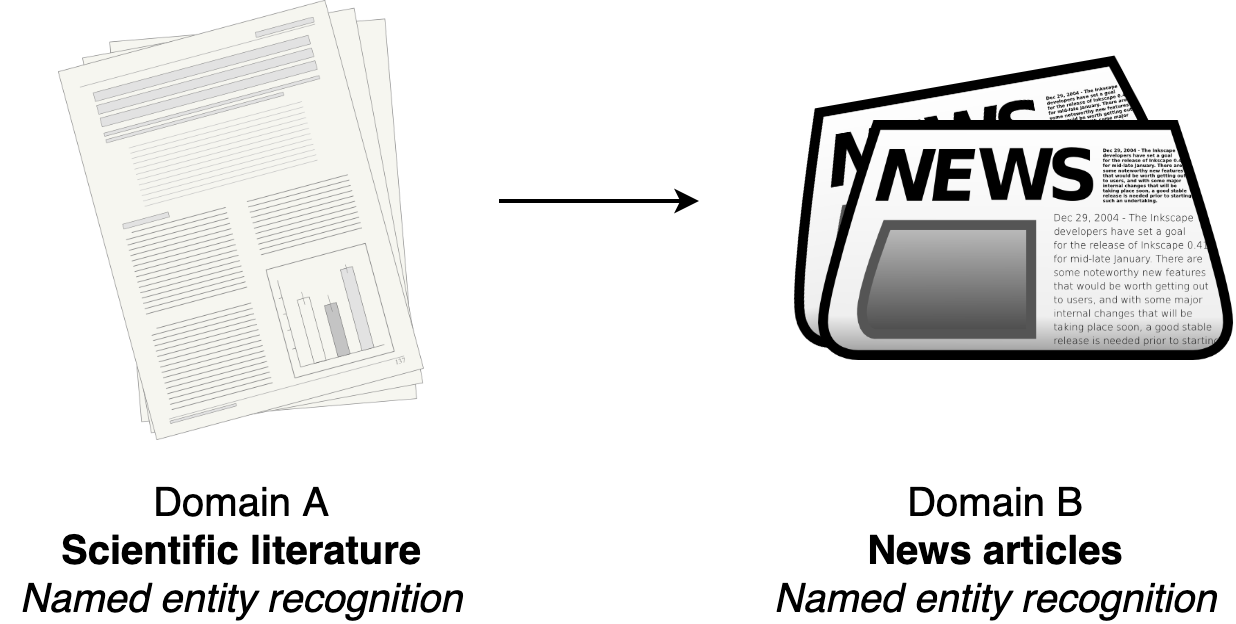
\includegraphics[scale=0.24]{0-img/domain-adaptation.png}
    \caption{An example domain adaptation problem, transferring knowledge from the domain of scientific literature to the domain of news articles, for the task of named entity recognition. Images sourced from Clker \cite{clker}.}
    \label{fig:domain-adaptation}
\end{figure}

Daumé \& Marcu \cite{daume} initially proposed the idea of `in-domain' and `out-of-domain' data, and applied these ideas to statistical learning theory. Other early work by Blitzer et al. \cite{scl} introduced the idea of structural correspondence learning, where ``pivot features'' are selected that occur frequently in both the source and target domain, and behave similarly in both. This correspondence can then help a classifier perform a task such as POS tagging on the target domain.

Pan et al. \cite{pan-sfa} proposed a spectral feature alignment algorithm that can group domain-specific words into clusters, based on the distances between the domain-independent words in the corpus. Domains-specific words are those that occur most frequently in one domain, whereas domain-independent words occur frequently in both domains. Michelbacher et al. \cite{feature-adaptation} consider domain-\{specific/independent\} features as a whole, and propose the idea of unsupervised feature adaptation for situations where no labelled target domain data is available. A classifier is trained on source domain data, and any domain-independent features are recomputed in an unsupervised fashion to align themselves with the target domain data, before being passed to the classifier to infer on the target domain data. Any domain-specific features are ignored.

The above methods all rely on some manual selection of features that are ``domain independent'' i.e. occur similarly in both the source and target domain. However, recent work has aimed to remove this manual step in the transfer learning process. Myagmar et al. \cite{cdsc} explored using BERT for cross-domain sentiment classification, finding that fine-tuning BERT on the source domain and running inference on the target domain (a process known as \textit{direct transfer}) beat several pre-existing benchmarks for the task, using significantly less training data and with much faster training times in addition.

Further work has been done to extend BERT for unsupervised domain adaptation. Ye et al. \cite{bert-feature-adaptation} use BERT's layer weights as features in a form of feature adaptation, and Du et al. \cite{domain-aware-bert} explore adding a post-training domain-distinguishing task to BERT's fine-tuning stages, and injecting adversarial learning into BERT.

Han \& Eisenstein propose AdaptaBERT \cite{adaptabert}, a novel unsupervised domain adaptation approach which adds an extra stage of masked language modelling on the target domain during fine-tuning. This gives a significant performance boost to the classifier, especially on words and phrases seen at inference time that were not seen in the source domain at training time (`out-of-vocabulary' terms). AdaptaBERT yields several percentage points higher accuracy than direct transfer methods for a historical English POS tagging task, with 30\% increase in accuracy on out-of-vocabulary terms. AdaptaBERT also outperforms existing methods on a Wikipedia $ \rightarrow $ Twitter transfer learning task.

Gururangan et al. \cite{dont-stop-pretraining} compared this approach, which they name task-adaptive pre-training, to a general domain-adaptive pre-training approach where MLM is performed on a large amount of generic target-domain text that is not necessarily aimed at the specific task at hand. They find a combination of both methods provides the highest classifier accuracy for transfer learning tasks between news articles, IMDB reviews and biomedical scientific papers.

\section{Going forward}

In this chapter we have defined political bias and looked at previous work in detecting political bias in the news with NLP and machine learning. We have discovered that ensemble classifiers are under-explored for this particular problem, which we examine further in Chapter \ref{chap:ensemble-bert}, where we also directly compare existing methods of detecting bias. We have also defined the related problem of readership bias and explored prior work in detecting readership bias on social media.

We then covered transfer learning and domain adaptation techniques. It is extremely rare to find social media content that has been annotated by political bias, due to the challenging nature of collecting annotations from real users, which is where the power of unsupervised domain adaptation comes in. Unsupervised domain adaptation methods don't need labels in the target domain, making them particularly suitable to the task of transferring between news articles and social media comments. However, for evaluation purposes we do end up needing to collected annotated social media data (see Chapter \ref{chap:reddit-data} for more on this).